\documentclass[10pt,twocolumn,preprint]{emulateapj}
\usepackage[english]{babel}
\usepackage{amsmath,color}

\newcommand{\bs}{\boldsymbol}
\newcommand{\diff}{{\mathrm d}}
\newcommand{\Cov}{\mathsf{C}}
\newcommand{\Fish}{\mathsf{F}}
\newcommand{\Cl}{\mathcal {C}}
\newcommand{\R}{\mathcal{R}}
\newcommand{\T}{\mathcal{T}}
\newcommand{\Msun}{M_\odot}

\newcommand{\tcb}{\textcolor{blue}}
\newcommand{\tcr}{\textcolor{red}}


\shortauthors{Yu et al.} \shorttitle{CUBE}
\begin{document}
\title{CUBE: A Memory-lite Cosmological $N$-body Algorithm}
\author{
Hao-Ran Yu$^{1,2}$,
Ue-Li Pen$^{2,3,4,5}$,
Xin Wang$^{2}$
}

\affil{
$^1$Tsung-Dao Lee Institute, Shanghai Jiao Tong University, Shanghai, 200240, China\\
$^2$Canadian Institute for Theoretical Astrophysics, University of Toronto, Toronto, ON M5H 3H8 Canada\\
$^3$Dunlap Institute for Astronomy and Astrophysics, University of Toronto, Toronto, ON M5S 3H4, Canada\\
$^4$Canadian Institute for Advanced Research, CIFAR Program in Gravitation and Cosmology, Toronto, ON M5G 1Z8, Canada\\
$^5$Perimeter Institute for Theoretical Physics, Waterloo, ON N2L 2Y5, Canada
}

\email{haoran@cita.utoronto.ca}
 
\begin{abstract}
Cosmological large scale structure $N$-body simulations are computation-light,
memory-heavy problems in supercomputing. Traditional $N$-body simulation
algorithms use at least 24-byte memory per particle, of which six 4-byte single 
precision floating point numbers keep track phase space coordinates of each particle.
Here we present the algorithm and accuracy of a new parallel, memory-lite, Particle-
Mesh based $N$-body code, where each particle can occupy as low as 6-byte memory. This 
is accomplished by storing relative position and relative velocity of each particle, 
in the format of 1-byte-integer, respect to their averaged value of a mesh-grid. The 
remaining information is given by complimentary density and velocity fields, which are 
negligible in memory space, and proper ordering of particles, which gives no extra 
memory. Our numerical experiments show that this integer based $N$-body algorithm 
provides acceptable accuracy compared to traditional algorithm in cosmological 
simulations. This significant lowering of memory-to-computation ratio breaks the 
bottleneck of scaling up and speeding up large cosmological $N$-body simulations on 
multi-core and heterogenous computing systems.

\end{abstract}

\keywords{}

\maketitle


\section{Introduction}\label{s.intro}
$N$-body simulation is a powerful tool to solve the highly nonlinear dynamic problems 
\citep{1988csup.book.....H}. It is widely used in cosmology to model the formation and 
evolution of the large scale structure (LSS). With the fast development of parallel 
supercomputers, we are able to simulate a system of more than a trillion ($10^{12}$) 
$N$-body particles. To date the largest $N$-body simulation in application is the 
``TianNu'' simulation \citep{2017NatAs...1E.143Y,2017RAA....17...85E} run on the 
TianHe-2 supercomputer by cosmological simulation code 
{\tt CUBEP3M} \citep{2013MNRAS.436..540H}. It uses nearly $3\times 10^{12}$ particles 
to simulate the cold dark matter (CDM) and cosmic neutrino evolution through the 
cosmic age.

The $N$-body simulations use considerable amount of memory, because the phase space 
coordinates $(x,y,z,v_x,v_y,v_z)$ of each $N$-body particle must be stored as, at 
least, six single precision floating point numbers (24 bytes). Contrarily, their 
computing workload can be alleviated by many algorithms, like Particle-Mesh [cite] and 
Tree [cite], scale as $o(N\log N)$ or even $o(N)$. On the other hand, modern 
supercomputer systems use multi cores, many integrated cores (MIC) and even densely 
parallelized GPUs, bringing orders of magnitude higher computing power, whereas these 
architectures usually have limited memory allocation. Thus, the computation-light but 
memory-heavy applications, compared to matrix multiplication and decomposition 
calculations, are less suitable for fully usage of the computing power of modern 
supercomputers. For example, although native and offload modes of {\tt CUBEP3M} are 
able to run on the Intel Xeon-PHI MIC architectures, with the require ment of enough 
memory, TianNu simulation were done on TianHe-2 with only its CPUs -- 73\% of the 
total memory but only 13\% of the total computing power.

We present a new $N$-body simulation code {\tt CUBE}, using as low as 6 byte
per particle (here after we use ``bpp'' referring to ``byte per particle'').
We show that it gives accurate results in cosmological LSS simulations.
The method is presented in \S\ref{s.method}, and a comparison between this method
and traditional method is shown in \S\ref{s.results}. Discussions and 
conclusions are in \S\ref{s.discussion}.

\section{Method}\label{s.method}
The most memory consuming part of a $N$-body simulation is usually the phase space 
coordinates of $N$-body particles -- 24 bpp (4 single precision floating numbers) must 
be used to store each particles' 3D position and velocity vectors. {\tt CUBEP3M}, an 
example of a memory-efficient parallel $N$-body code, can use as low as 40 bpp in 
sacrificing computing speed \citep{2013MNRAS.436..540H}. This includes the phase 
coordinates (24 bpp) for particles in physical domain and buffered region, a linked 
list (4 bpp), and a global coarse mesh and local fine mesh. 4-byte real numbers are 
not necessarily adequate in representing the {\it global} coordinates in simulations.
If the box size is many orders of magnitude larger than interactive distance
between particles, especially in the field of re-simulation of dense subregions,
double precision (8-byte) coordinates are needed to avoid truncation errors.
Another solution is to record {\it relative} coordinates for both position and velocity.
{\tt CUBE} replaces the coordinates and linked list 24+4=28 bpp memory usage
with an integer based storage, reduces the basic memory usage from 28 bpp down to
6 bpp, described as following \ref{ss.position} and \ref{ss.velocity}. The algorithm is described in \ref{ss.overview}.

\subsection{Particle position storage}\label{ss.position}
We construct a uniform mesh throughout the space and each particle belongs 
to its parent cell of the mesh. Instead of storing global coordinates of 
each particle, we store its offset relative to its parent cell which 
contains the particle. We divide the cell, in each dimension $d$, evenly into 
$2^8=256$ bins, and use a 1-byte (8 bits) integer $\chi_d \in \{-128,-127,...,127\}$ to 
indicate which bin it locates in this dimension. The global locations of 
particles are given by cell-ordered format in memory space, and a 
complimentary number count of particle number in this mesh (density field) 
will give complete information of particle distribution in the mesh. Then 
the global coordinate in $d$th dimension $x_d$ is given by $x_d=(n_c-1)+
(\chi_d+128+1/2)/256$, where $n_c=1,2,...,N_c$ 
is the index of the coarse grid. The mesh 
is chosen to be coarse enough such that the density field takes negligible 
memory. This coarse density field can be further compressed into 1-byte 
integer format, such that a 1-byte integer show the particle number in this 
coarse cell in range 0 to 255. In the densest cells (rarely happened) where 
there are $\ge 255$ particles, we can just write 255, and write the actual 
number as a 4-byte integer in another file.

In a simulation with volume $L^3$ and $N_c^3$ coarse cells, particle 
positions are stored with a precision of $L/(256N_c)$. The force calculation 
(e.g. softening length) should be configured much finer than this 
resolution, discussed in later sections. On the other hand, particle 
position can also be stored as 2-byte (16 bits) integers to increase the resolution. 
In this case, each coarse cell is divided into $2^{16}=65536$ bins and the 
position precision is $L/(65536N_c)$, precise enough compared to using
4-byte global coordinates, see later results. We denote this case ``x2'' and 
denote using 1-byte integers for positions ``x1''.

We collectively write the general position conversion formulae
\begin{equation}\label{eq.chi}
	\chi_d=\left[2^{8n_\chi}(x_d-\left[x_d\right])\right]-2^{8n_\chi-1},
\end{equation}
\begin{equation}\label{eq.x}
	x_d=(n_c-1)+2^{-8n_\chi}\left(\chi_d+2^{8n_\chi-1}+1/2\right),
\end{equation}
where $[\ ]$ is the operator to take the integer part. $n_\chi\in\{1,2\}$ is the number of bytes used for each integer, $x_d$ and $\chi_d$ are floating and integer version of the coordinate. The velocity counterpart of them are $n_\nu=1,2$, $v_d$ and $\nu_d$. $n_c=1,2,...$ is the coarse grid index, given by the ordering of particles and a integer based particle density field (see \ref{sss.spatial_decomposition}). The position resolution for $n_\chi$-byte integer, ``x$n_\chi$'', is $2^{-8n_\chi}L/N_c$.

As a $n_\chi=1$, 1D ($d=1$), 4-coarse-cell ($N_c=4$) example, if $$\chi_1=(-128,127,0,60),$$ particle number density $${\rho_c^{\rm 1D}}=(1,0,2,1),$$ then in unit of coarse cells, $$x_1=(0.001953125, 2.998046875, 2.501953125, 3.736328125).$$

\begin{figure}
\centering
  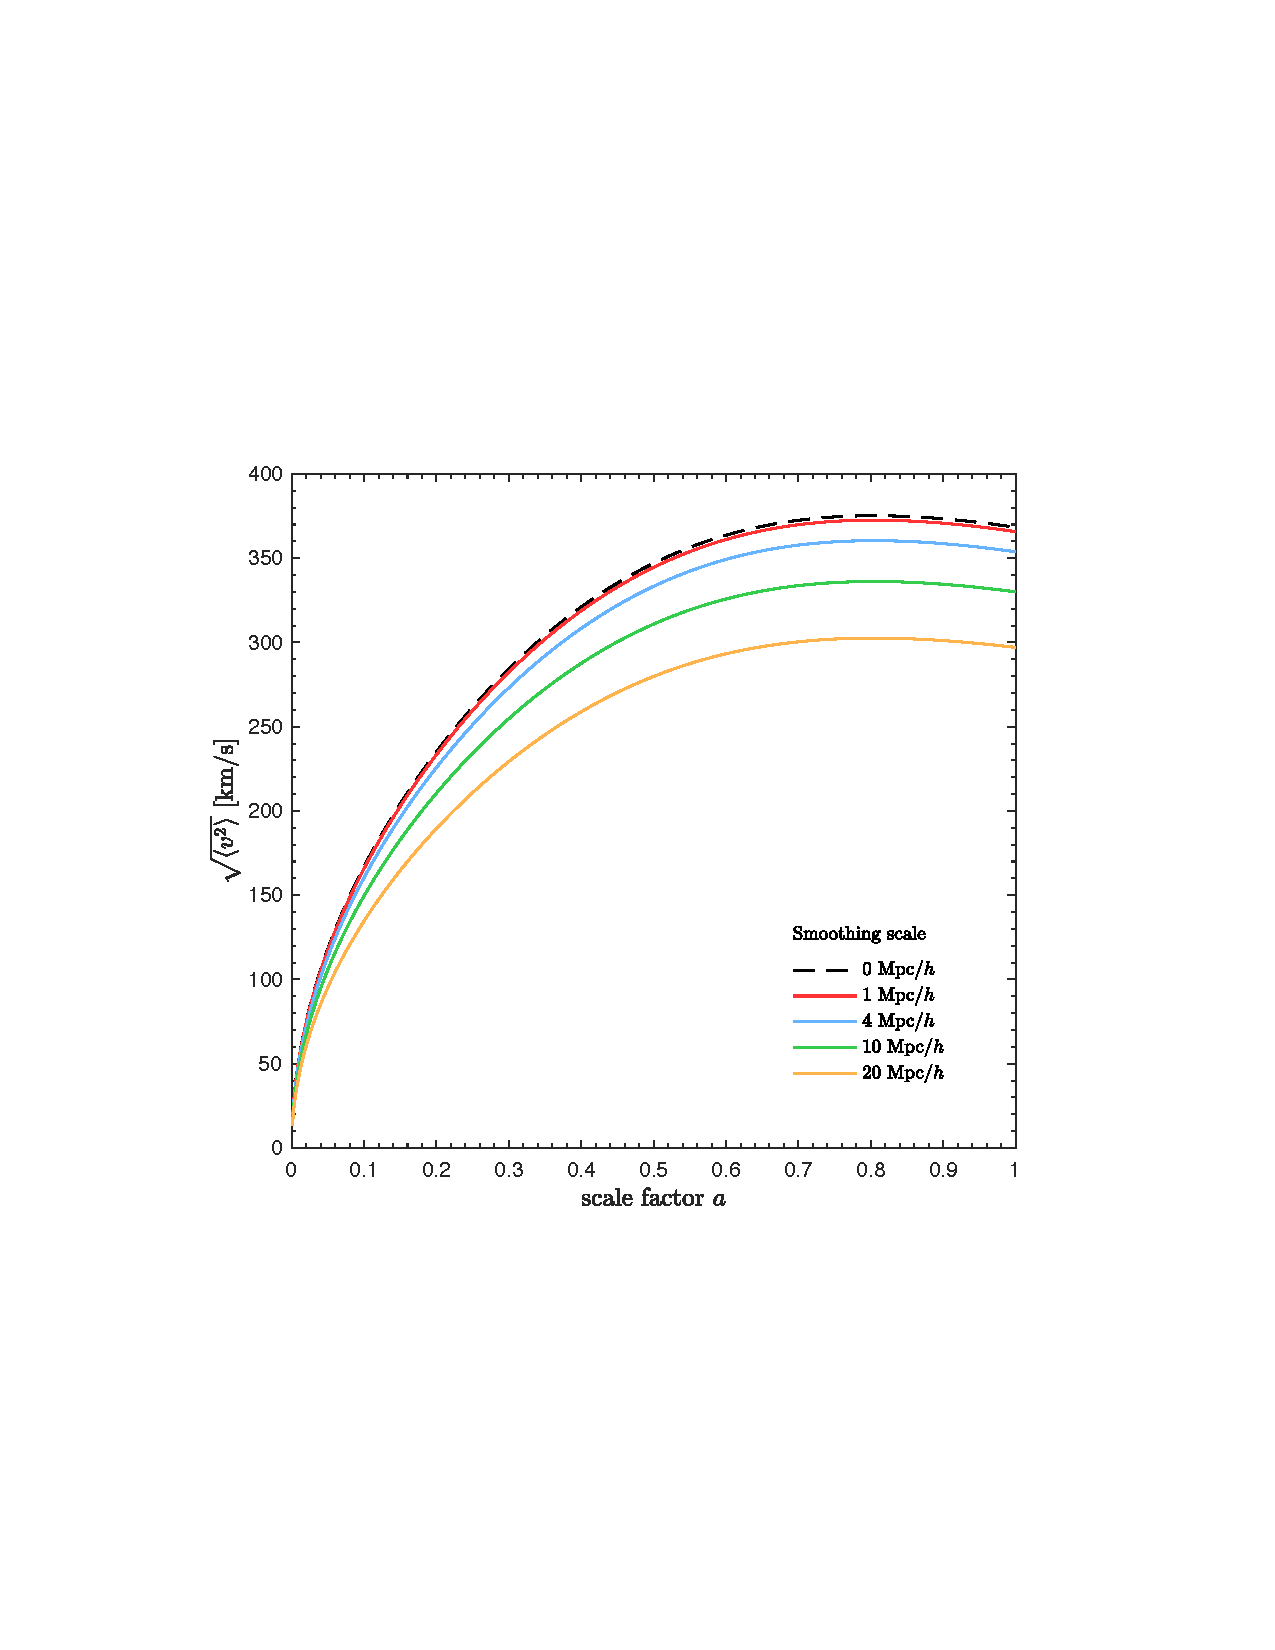
\includegraphics[width=1.0\linewidth]{vdisp.pdf}
 \caption{\tcb{Xin, could you please check the units of both $y$-axis?}}
\label{fig.vdisp}
\end{figure}

\subsection{Particle velocity storage}\label{ss.velocity}
Similarly, actual velocity in $d$th dimension $v_d$ is decomposed into an 
averaged velocity field on the same coarse grid $v_c$ and a residual $\Delta v$ 
relative to this field: 
\begin{equation}
	v_d=v_c+\Delta v.
\end{equation}
$v_c$ is always recorded and 
kept updated, and occupies negligible memory. We then divide velocity space 
$\Delta v$ into uneven bins, and use a $n_\nu$-byte integer to indicate
which $\Delta v$ bin the particle is located.

The reason why we use uneven bins is that, slower particles are more 
abundant compared to faster ones, and one should better resolve slower 
particles tracing at least linear evolution. On the other hand, there could 
be extreme scattering particles (in case of particle-particle force), and we 
can safely ignore or less resolve those nonphysical particles. One of the 
solution is that, if we know the probability distribution function (PDF) 
$f(\Delta v)$ we divide its cumulative distribution function (CDF) $F(\Delta 
v)\in(0,1)$ into $2^{8n_\nu}$ bins to determine the boundary of $\Delta v$ 
bins, and particles should evenly distribute in the corresponding uneven $
\Delta v$ bins. Practically we find that either $f(v_d)$ or $f(\Delta v)$ is 
close to Gaussian, so we can use Gaussian CDF, or any convenient analytic 
functions which are close to Gaussian, to convert velocity between real 
numbers and integers.

The essential parameter of the velocity distribution is its variance. On 
non-linear scale, the velocity distribution function is non-Gaussian. 
However, to the first order approximation, we simply assume it as Gaussian 
and characterized by the variance
\begin{equation}\label{eq.vdisp}
	\tcb{ \sigma_v(a,k) = \frac{1}{3}  (a H f D)^2 \int_0^kd^3q\frac{P_{L}(q)}{q^2}},
\end{equation}
where $a(z)$ is the scale factor, $H(z)$ the Hubble parameter, $D$ is the 
linear growth factor, $f=d \ln D/d\ln a$, and $P_L(k)$ is the linear power 
spectrum of density contrast at redshift zero.
$\sigma_v(a,k)$ is a function of cosmic evolution $a$ and a smoothing scale 
$k$, or $r$ (see Figure \ref{fig.vdisp}). $\Delta v$
is the velocity dispersion relative to the coarse grid, so we approximate 
its variance as
\begin{equation}\label{eq.vdelta}
	\sigma^2_{\Delta}(a)=\sigma^2_v(a,r_c)-\sigma^2_v(a,r_p), 
\end{equation}
where $r_c$ is the scale of
coarse grid, and $r_p$ is the scale of average particle separation. In each
dimension of 3D velocity field, we use $\sigma^2_{\Delta}(a)/3$ according 
to the equipartition therorem. On different scales, we measure the 
statistics of $v_d$, $v_c$ and $\Delta v$ and find good agreement with the 
above model.

\begin{figure}
\centering
  \includegraphics[width=0.95\linewidth]{fig_tile.pdf}
 \caption{Spacial decomposition in {\tt CUBE} in a 2D analogy. In this example, there are 2 images per dimension (${\tt nn}=2$), and 2 tiles per image per dimension (${\tt nnt}=2$). The orange boxes show the overlapped physical+buffer regions, inside of which one physical regions is indicated with green.}
\label{fig.tile}
\end{figure}

The simulation results are very insensitive if we manually tune the variance of the model $\sigma_\Delta$ within an order of magnitude. However, in $n_\nu=1$ case, the method of using uneven bins gets much better results than simply using equal bins between minimum and maximum values $[\min(\Delta v),\max(\Delta v)]$. So, one can safely use a standard $\Lambda$CDM (cold dark matter with a cosmological constant as dark energy) for slightly different cosmological models, in equation (\ref{eq.vdisp}). In {\tt CUBE}, the velocity conversion takes the formula
\begin{equation}\label{eq.nu}
	\nu_d=\left\lfloor(2^{8n_\nu}-1)\pi^{-1}\tan^{-1}\left((v_d-v_c)\sqrt{\pi/2\sigma_\Delta^2}\right)\right\rfloor,
\end{equation}
\begin{equation}\label{eq.v}
	v_d=v_c+\tan\left(\frac{\pi\nu_d}{2^{8n_\nu}-1}\right)\sqrt{2\sigma_\Delta^2/\pi},
\end{equation}
where $\lfloor\ \rfloor$ is the operator to take the nearest integer. 
Tangent functions are convenient and compute very fast. Compared to error 
functions used in Gaussian case, they take the same variance at $\nu_d=0$ but 
resolve high velocities relatively better.
Note again that proper choice of conversion formulae and $\sigma_\Delta$ 
only optimizes the velocity space sampling, but does not affect the physics. 

Initially, particles are generated by initial condition generator, at a higher redshift. The coarse grid density field $v_c$ is also generated at this step by averaging all particles in the coarse cell. A global $\sigma_\Delta$ is calculated by equation (\ref{eq.vdelta}), where linear approximation is hold. Then velocities are stored by equation (\ref{eq.nu}). During the simulation, $v_c$ is updated every time step, and a nonlinear $\sigma_\Delta$ is measured directly from the simulation, and can be simply used in the next time step, after scaled by the ratio of growth factors between two adjacent time steps. More details see section \ref{sss.algorithm}.

\subsection{Code overview}\label{ss.overview}
{\tt CUBE} uses a 2-level PM force calculation, same as {\tt CUBEP3M}, However, in order to apply the integer based format to the $N$-body simulation, substantial structural changes need to be done. {\tt CUBE} is written in Coarray Fortran, where Coarray features implement MPI communication between computation nodes/images\footnote{Images are the concept of computing nodes or MPI tasks in Coarray Fortran. We use this terminology in this paper.}.
The algorithm is described in this language. 

\subsubsection{Spacial decomposition}\label{sss.spatial_decomposition}
{\tt CUBE} uses cubic decomposition structures. The global simulation volume is decomposed into ${\tt nn}^3$ cubic sub-volumes with {\tt nc} coarse grids per side, and each of these are assigned to a coarray {\it image}. Inside of an image, the sub-volume is further decomposed into ${\tt nnt}^3$ cubic {\it tiles}, with {\tt nt}={\tt nc}/{\tt nnt} coarse grids per side, which is a essential unit in the calculations. Each tile is surrounded by a {\it buffer} region which is ${\tt ncb}$ coarse cells thick. The buffer is designed for two reasons: (1) computing the fine mesh force, whose cut-off length ${\tt nforce\_cutoff}\leq{\tt ncb}$, and (2) collecting all possible particles travelling from a tile's buffer region to its center, {\it physical} region. Figure \ref{fig.tile} shows the spacial decomposition in a 2-dimensional analogy, with ${\tt nn=2}$ and ${\tt nnt=2}$. According to this spatial decomposition, and as discussed in the last two subsections, we declare $\{\rho_c,\chi_d,v_c,\nu_d\}$, or in variable expression $\{{\tt rho\_c},{\tt xp},{\tt vfield},{\tt vp}\}$ as follows:
\begin{eqnarray*}
	&&{\tt integer(1)\ rho\_c(nex,nex,nex,nnt,nnt,nnt)[nn,nn,*]}\\
	&&{\tt integer(}n_\chi{\tt )\ xp(npmax)[nn,nn,*]}\\
	&&{\tt real(4)\ vfield(nex,nex,nex,nnt,nnt,nnt)[nn,nn,*]}\\
	&&{\tt integer(}n_\nu{\tt )\ vp(npmax)[nn,nn,*]}
\end{eqnarray*}
where ${\tt nex}={\tt nt}+2\times{\tt ncb}$ covers the buffer region on both sides, {\tt nnt} is the tile dimemsions, and {\tt nn} is the image {\it codimensions}\footnote{Coarray Fortran concept. Codimensions can do communications between images.}. We denote actual number of particles in a given image {\tt nplocal}, and ${\tt npmax}>{\tt nplocal}$ is a value (discussed in Section \ref{ss.memory}) large enough to store particles. The particle position and velocity arrays {\tt xp} and {\tt vp} (equivalent to $\chi_d$ and $\nu_d$ in \ref{ss.position} and \ref{ss.velocity} respectively) are required to be sorted according to the same memory layout of {\tt rho\_c}, such that $n_c$ and thus global positions of particles $x_d$ can be obtained by equation (\ref{eq.x}). $\{{\tt rho\_c},{\tt xp},{\tt vfield},{\tt vp}\}$ provides a complete information of positions and velocities of particles, and we call it a snapshot, or checkpoint.


\subsubsection{Algorithm}\label{sss.algorithm}
Figure \ref{fig.code} shows the overall structure of the code and these subroutines are described in following paragraphs. 

{\tt initialize} and {\tt read\_particles} -- The subroutine {\tt initialize} creates necessary FFT plans and read in configuration files telling the program at which redshifts we need to do checkpoints, halofinds, or stop the simulation. Force kernels {\tt kern\_c}, {\tt kern\_f} are also created or read in here. In {\tt read\_particles}, for each image, we read in all particles in {\it physical} regions of every tile (indicated in Figure \ref{fig.tile}), i.e., $\{{\tt rho\_c},{\tt xp},{\tt vfield},{\tt vp}\}$. These are obtained by the initial condition generator (see Appendix A). Because physical regions of tile are {\it complete} and {\it disjoint} in space, particles at this stage are also complete and disjoint. We call it ``disjoint state''. At this stage, {\tt rho\_c}'s buffer regions of each tile are 0, and the elements of {\tt xp} and {\tt vp} beyond physical number -- {\tt xp(nplocal+1:)} and {\tt vp(nplocal+1:)} can be arbitrary and are not used.

{\tt buffer\_density}, {\tt buffer\_x} and {\tt buffer\_v} -- In order to use the integer based format, {\tt xp} and {\tt vp} must always be ordered, and their number density field {\tt rho\_c} must always be present. In updating arrays of {\tt xp} and {\tt vp} (not simultaneously) of a local tile, a vicinity (buffer) region of the physical region is also needed. First, buffer regions of {\tt rho\_c} is synchronized between tiles and images by subroutine {\tt buffer\_density}. Then, by subroutines {\tt buffer\_x} and {\tt buffer\_v} respectively, {\tt xp} and {\tt vp} are updated to contain common, buffered particles, in an order according to the new, buffered {\tt rho\_c}. We call this stage ``buffered state''. After {\tt particle\_initialize} is done by all images (synchronized by a ``{\tt sync all}'', which is equivalent to a {\tt mpi\_barrier}), these three subroutines are called and particles are converted from disjoint state to buffered state.

\begin{figure}[t]
\begin{verbatim}

    program CUBE
      call initialize
      call read_particles
      call buffer_density
      call buffer_xp
      call buffer_vp
      do
        call timestep
        call update_xp
        call buffer_density
        call buffer_xp
        call update_vp
        call buffer_vp
        if(checkpoint_step) then
           call update_xp
           call checkpoint
           if (final_step) exit
           call buffer_density
           call buffer_xp
           call buffer_vp
        endif
      enddo
      call finalize
    end
\end{verbatim}
\caption{Overall structure of {\tt CUBE}.}
\label{fig.code}
\end{figure}


{\tt timestep} --
We operate a Runge-Kutta 2 method for time integration. i.e., we update position ($D$=drift) and velocity ($K$=kick) every half time step. For $n$ time steps, the operation would be $(DKKD)^n$ which is 2nd order accurate. The actual simulation applies varied time steps. In each iteration of the main loop, we firstly call {\tt timestep}, where a increment of time {\tt dt} is controlled by particles' maximum velocities, accelerations, cosmic expansion and any other desired conditions.

{\tt update\_xp} --
According to {\tt dt}, subroutine {\tt update\_xp} updates the positions of particles in a ``{\it gather}'' algorithm (in contrast, {\tt CUBEP3M} uses ``scatter'' algorithm) tile by tile. For each particle, {\tt xp} and {\tt vp} are converted to $x_d$ and $v_d$ by Equations(\ref{eq.x},\ref{eq.v}). Because each tile is in the buffered state with buffer depth {\tt ncb}, we are able to collect all possible particles whose $v_d\times{\tt dt}<{\tt ncb}$ from physical+buffer region to its physical region.

In order to keep particles ordered, for each tile, we first do $x_d=x_d+v_d\times{\tt dt}$ on all particles to obtain an updated density and velocity field on the tile, {\tt rho\_c\_new} and {\tt vfield\_new}. Then, this calculation in done on the same tile again\footnote{This repetition scales as $o(N)$ and is computational inexpensive.} to generate a new, local particle list {\tt xp\_new} and {\tt vp\_new} on the tile by Equations(\ref{eq.chi},\ref{eq.nu}). Here, the ordering of particles depends on {\tt rho\_c\_new}, and {\tt vfield\_new} is used as $v_c$ in Equation(\ref{eq.nu}). Then, another iteration is done on this tile to discard buffer regions of $\{{\tt rho\_c\_new},{\tt xp\_new},{\tt vfield\_new},{\tt vp\_new}\}$, converting buffer state to disjoint state, and it replaces corresponding part of $\{{\tt rho\_c},{\tt xp},{\tt vfield},{\tt vp}\}$. When all tiles are iterated, the entire image is in disjoint state, and {\tt nplocal} is updated. Then all images is synchronized by {\tt sync all} and we sum up {\tt nplocal} over images to check if total number of particles {\tt npglobal} is conserved. These steps are summarized in Figure \ref{fig.update_xp}.

\begin{figure}[t]
\begin{verbatim}

subroutine update_xp
  do (each tile)
    do (each coarse grid)
      do (each particle)
        calculate particle's new coarse grid position
        update rho_c_new
        update vfield_new
      enddo
    enddo
    do (each coarse grid)
      do (each particle)
        calculate particle's new accurate position
        calculate particle's index
        update xp_new(index) & vp_new(index)
      enddo
    enddo
    do (each coarse grid)
      discard buffer information
      replace xp and vp for this tile
    enddo
  enddo
  sync all
  update velocity dispersion
  check nplocal & npglobal
end
\end{verbatim}
\caption{Pseudocode for subroutine {\tt update\_xp}.}
\label{fig.update_xp}
\end{figure}

\begin{figure}[t]
\begin{verbatim}

subroutine update_vp
  do (each tile)
    calculate fine mesh density
    calculate fine mesh force: local FFT
    update fine mesh velocity
    update maximum acceleration
    if (PP force) then
      PP calculation & velocity update
      update maximum acceleration
    endif
  enddo
  sync all
  calculate coarse mesh density
  calculate coarse mesh force: global pencil FFT
  update coarse mesh velocity
  update maximum acceleration
  update maximum velocity
end
\end{verbatim}
\caption{Pseudocode for subroutine {\tt update\_vp}.}
\label{fig.update_vp}
\end{figure}

{\tt update\_vp} -- 
After {\tt update\_xp}, or drift $D$, we call {\tt buffer\_density} and {\tt buffer\_xp} in order that particle positions are in buffered state, based on which, we update velocities (kick $K$) of particles in physical region of each tile. {\tt CUBE} uses a 2-level particle mesh scheme \citep{2013MNRAS.436..540H}. Local fine forces have a force cutoff ${\tt nforce\_cutoff}\leq{\tt ncb}$, i.e., $F_{\rm fine}(r>{\tt ncb})=0$. So, if we apply a fine-grid particle-mesh on an extended tile with buffered-depth {\tt ncb} (see Figure \ref{fig.tile} and regard it periodic), the force on physical regions does not depend on the false periodic boundary assumption, and the resulting fine force $F_{\rm fine}$ and velocity update on physical region is correct.


The compensating coarse grid force $F_{\rm coarse}$ is globally computed by using a coarser (usually by factor of 4) mesh by dimensional splitting -- a distributed-memory cubic decomposed 3D coarse density field is interpolated by particles, and we Fourier transform data in consecutive three dimensions with global transposition in between (known as the pencil decomposition). After the multiplication of force kernels, the inverse transform takes place to get the cubic distributed coarse force field $F_{\rm coarse}$, upon which velocities are updated again.

An optional particle-particle (PP) force $F_{\rm pp}$ can be called to increase the force resolution and the velocities are updated again. The collective operations of velocity update is Equation(\ref{eq.v}), $v_d=v_d+F_{\rm total}$ and Equation(\ref{eq.nu}).

The maximum accelerations $\max(\dot{v}_{\rm fine})$, $\max(\dot{v}_{\rm coarse})$, $\max(\dot{v}_{\rm pp})$ and maximum of velocities $\max(v_d)$ are collected controlling {\tt dt} for the {\tt timestep} in the next iteration. We also update $\sigma^2_{\Delta}$ according to the new $v_d-v_c$.

By far, {\tt vp} in physical regions are correctly updated. Remember that particle locations in the buffer regions has updated before {\tt PM} and remained unchanged. So we simply call {\tt buffer\_v} again such that the {\tt update\_x} in the next iteration will be done correctly. We call {\tt update\_vp} to convert {\tt vp} into buffered state. These steps are summarized in Figure \ref{fig.update_vp}.

{\tt checkpoint} -- 
If a desired redshift is reached, we execute the last drift step in the $(DKKD)^n$ operation by {\tt update\_xp}, and call {\tt checkpoint} to save the disjoint state of \{{\tt xp}, {\tt vp}, {\tt rho\_c}, {\tt vfield}\} on disk. Related operations, like run-time halo finder, projections are also done at this point. If final desired redshift is reached, {\tt final\_step} let us exit the main loop. These corresponding logical variables are controlled in {\tt timestep}.

{\tt finalize} --
Finally, in {\tt finalize} subroutine we destroy all the FFT plans and finish up any timing or statistics taken in the simulation.

\subsection{Memory layout}\label{ss.memory}
Here we list the memory-consuming arrays and how they scale with different configurations of the simulation. We classify them into (1) arrays of particles, (2) coarse mesh arrays and (3) fine mesh arrays.

\subsubsection{Arrays of particles}
The arrays of particles contains {\tt xvp(6,npmax)} and a temporary {\tt xvp\_new(6,nptile)}\footnote{We use ``{\tt xvp}'' to represent $\{{\tt xp},{\tt vp}\}$, and use ``{\tt xvp\_new}'' to represent $\{{\tt xp\_new},{\tt vp\_new}\}$.}. {\tt npmax} is the number of particles {\tt xvp} can store:
\begin{equation}\label{eq.npmax}
	{\tt npmax}=\left\langle {\tt nplocal} \right\rangle \left( 1+\frac{2\times {\tt ncb}}{\tt nt} \right)^3(1+\epsilon_{\rm image}),
\end{equation}
where $\left\langle {\tt nplocal} \right\rangle$ is the average number of particles per image. The second term above let us store particles in buffer regions, and the third term $1+\epsilon_{\rm image}$ takes into account the inhomogeneity of {\tt nplocal} on different images. When each image models smaller physical scales, $\epsilon_{\rm image}$ should be set larger. 

{\tt xvp\_new} stores temporary particles only on tiles:
\begin{equation}\label{eq.nptile}
	{\tt nptile}=\left\langle {\tt nplocal} \right\rangle \left( \frac{1}{\tt nnt} \right)^3(1+\epsilon_{\rm tile}),
\end{equation}
where, recall that {\tt nnt} is the number of tiles per image per dimension, and similarly $\epsilon_{\rm tile}$ controls the inhomogeneity on scale of tiles. Larger {\tt nnt} causes more inhomogeneity on smaller tiles, and $\epsilon_{\rm tile}$ can be much larger than $\epsilon_{\rm image}$, however the term ${\tt nnt}^{-3}$ decreases much faster. So, the majority memory is occupied by {\tt xvp}.

\subsubsection{Coarse mesh arrays}
On coarse mesh, {\tt rho\_c}, {\tt vfield} and force kernel {\tt kern\_c} should always be kept. They are usually configured to be 4 times coarser than fine grids and particle number density. In this case, each coarse grid, 3D {\tt vfield} takes only 12 bytes, and 64 particles will at least take 384 bytes ($n_\chi=n_\nu=1$ case). Similarly, pencil-FFT arrays, coarse force arrays etc. are memory-light and/or temporary.

\subsubsection{Fine mesh arrays}
On the local fine mesh, only a force kernel array needs to be kept. The fine mesh density arrays, force field arrays are temporary. Since {\tt xvp\_new}, coarse force arrays, pencil-FFT arrays are also temporary and are not used in any calculation simultaneously, they can be overlapped in memory by using equivalent statements.

\begin{table}[]
\centering
\caption{Memory layout for a certain configuration}
\label{t.memory}
\begin{tabular}{llrrr}
\hline
& & \multicolumn{3}{c}{Memory usage}\\
\cline{3-5}
Type     & Array & /GB & /bpp & Percentage \\
\hline
Particles  & \tt xvp          & 29.9   & 8.24   & 83.8\%     \\
           & \tt xvp\_new     & \underline{3.16}   & \underline{0.872}  & \underline{8.87\%}     \\
           & \tt PID          & 0      & 0      &    0\%     \\
           & Subtotal         & 33.0   & 9.12   & 92.7\%     \\
\hline
Coarse mesh& \tt rho\_c       & 0.296  & 0.0818 & 0.831\%    \\
           & \tt vfield       & 0.889  & 0.245  & 2.49\%     \\
           & \tt kern\_c      & 0.340  & 0.0939 & 0.954\%    \\
           & \tt force\_c     & (0.690)  & (0.190)  & (1.94\%)    \\
           & \tt rho\_c\_new  & 0.0140 & 0.00388  & 0.0394\% \\
           & Pencil-FFT       & (0.454)  & (0.125) & (1.27\%)      \\
           & Subtotal         & 1.55   & 0.429 & 4.36\%     \\
\hline
Fine mesh  & \tt kern\_f      & 1.06   & 0.292 & 2.97\%      \\
           & \tt force\_f     & (1.63) & (0.450) & (4.57\%)     \\
           & Fine-FFT     &   (1.41) & (0.389) & (3.96\%)     \\
           & Subtotal      & 1.06   & 0.292 & 2.97	\%      \\
\hline
Total &                      & 35.6 & 9.84 & 100\%\\
\hline
\multicolumn{2}{l} {Optimal limit} & 21.7 & 6 & 61.0\%\\
\hline
\end{tabular}
\end{table}

\subsubsection{Compare with traditional algorithms}
To illustrate the improvement of memory usage, we give an example of TianNu simulation \citep{2017NatAs...1E.143Y} on the Tianhe-2 supercomputer, which used a traditional {\tt CUBEP3M} code. TianNu's particles number is limited by memory per computing node -- per computing node, an average of $576^3$ neutrino particles and $288^3$ CDM particles are used, and consumes about 40 GB of memory\footnote{Additional memory is used for OpenMP parallelization and for particle IDs to differentiate different particle spices.}, or about 186 bpp. A memory efficient case of {\tt CUBEP3M} by using large physical scales and at costs of speed, still uses about 40 bpp. 

By using {\tt CUBE}, with parameters $n_\chi=n_\nu=1$, ${\tt nc}=384$, ${\tt nnt}=3$, ${\tt ncb}=6$, $\epsilon_{\rm image}=5\%$, $\epsilon_{\rm tile}=200\%$ and $\left\langle {\tt nplocal} \right\rangle=1536^3$, we use about 35.6 GB of memory, corresponding to 9.84 bpp. This can be done on most of the supercomputers, even modern laptops.

Table \ref{t.memory} shows the memory consumption for this test simulation. The memory-consuming arrays are listed and classified into the three types above mentioned, and their memory usages are in unit of GB ($10^9$ bytes), byte per particle (bpp), and their percentage to the total memory usage. The parenthesized numbers show overlapped memory, which is saved by equivalencing them with the underscored numbers. There are other, unlisted variables which are memory-light, and can also be equivalenced with listed variables. For this $1536^3$ per image simulation, using ${\tt nnt}^3=27$ tiles per image optimizes the memory usage, because it well controls the balance between the second terms in Equations (\ref{eq.npmax},\ref{eq.nptile}). A great amount of temporary memory in coarse and fine mesh force calculations is equivalenced to {\tt xvp\_new}.

In the bottom of Table \ref{t.memory} we stress that the optimal memory usage is 6 bpp, or 21.7 GB, 61\% of the actual memory usage in this test simulation. The most prominent departure from this limit is that {\tt xvp} already uses 8.24 bpp, and all other variables occupy only additional 8\%. Of coarse, on modern super computers, the memory per computing node is usually much larger, by scaling up the number of particles per node, the buffer ratio ${\tt ncb}/{\tt nt}$ will be lowered and we can approach closer to the 6 bpp limit.

\section{Accuracy}\label{s.results}
We run a group of simulations to test the accuracy of {\tt CUBE}. We use same seeds to generate same Gaussian random fields in the initial condition generators of {\tt CUBEP3M} and {\tt CUBE}, and then they produce initial conditions of their own format respectively. Then the main $N$-body codes run their own initial conditions to redshift $z=0$.

First, by using different configurations -- different number of computing nodes, box sizes, particle resolutions, different number of tiles per node/image etc., we find that by using 2-byte integers for both positions and velocities ($n_\chi=n_\nu=2$, or x2v2) {\tt CUBE} gives exact results compared to {\tt CUBEP3M}. So, if memory usage is not a problem, one can always double the memory usage to get exact results, and the optimal memory limit of this case is 12 bpp, still much lower than traditional methods. Next, we focus on the accuracy of the other three cases -- x1v2, x2v1 and x1v1.

We list the names and configurations of simulations used in Table \ref{t.sim}, where $N_{\rm image}$, $L$, $z_i$, $z_{\rm checkpoint}$ and $N_p$ are respectively the number of computing nodes used, length of the side of the box, initial redshift, redshift where we do checkpoint and total number of particles. These configurations are run by {\tt CUBEP3M}, x2v2, x1v2, x2v1 and x1v1 versions of {\tt CUBE}. Using different number of tiles per image gives exact same results.

\begin{table}[]
\centering
\caption{Simulation configurations}
\label{t.sim}
\begin{tabular}{lrrrrr}
\hline
& \multicolumn{5}{c}{Configurations}\\
\cline{2-6}
Name  & $N_{\rm image}$ & $L/(h^{-1}{\rm Mpc})$ & $z_i$ & $z_{\rm checkpoint}$ & $N_p$ \\
\hline
S512   & 8     & 200.0   & 49.0 & 0      & $512^3$     \\
S256   & 1     & 80.0    & 49.0 & 0      & $256^3$     \\
S2048S & 64    & 300.0   & 49.0 & 1.0, 0  & $2048^3$     \\
S2048L & 64    & 1200.0  & 49.0 & 1.0, 0  & $2048^3$     \\
\hline
\end{tabular}
\end{table}

\begin{figure}[t]
\centering
  \includegraphics[width=0.95\linewidth]{overplotparticles.pdf}
 \caption{Difference between using {\tt CUBEP3M} (grey dots) and {\tt CUBE}-x1v1 (red dots). The box shows a projected $15.625^2\times 3.90625\ ({\rm Mpc}/h)^3$ region of the simulation. }
\label{fig.particles}
\end{figure}

\subsection{Displacement of particles}
In S512, we zoom into a small region of $15.625^2\times 3.90625\ ({\rm Mpc}/h)^3$ and compare the particle distribution between {\tt CUBEP3M} and {\tt CUBE}-x1v1 in Figure \ref{fig.particles}. For clarity, {\tt CUBEP3M} particles are marked with bigger, grey dots, whereas smaller red dots are {\tt CUBE}-x1v1 particles over-plotted onto them. One can see the difference between them. 1 ${\rm Mpc}/h$, fine grid and coarse grid scales are shown in the figure. The position resolution of particles in {\tt CUBE}-x1v1 is 1/256 of a coarse grid, or 1/64 of a fine grid.

To quantify the offset in the final particle distributions, we use PIDs to track the displacement ${\bs \Psi}({\bs q})\equiv{\bs x}-{\bs q}$ of every particle \citep{2017PhRvD..95d3501Y}, where ${\bs x}$ and ${\bs q}$ are Eulerian and Lagrangian coordinates of the particle. Then we calculate the absolute value of the offset vector
\begin{equation}\label{eq.offset}
	\Delta\Psi\equiv|{\bs\Psi}_i-{\bs\Psi}_0|.
\end{equation}
Here, ${\bs\Psi}_0$ stands for {\tt CUBEP3M} and subscript $_i$ can stand for x2v2, x1v2, x2v1 or x1v1. The probability distribution functions (PDFs) and cumulative distribution functions (CDFs) of $\Delta\Psi$ in S256 are shown in Figure \ref{fig.dsp}. Results from x2v2, x1v2, x2v1 or x1v1 are in black, red, blue and green respectively. The results from absolute displacement of particles (by replacing ${\bs\Psi}_i$ with ${\bs q}$ in Equation (\ref{eq.offset})) are shown in grey for comparison.

For x2v2, almost all particles are accurate up to 1/100 of a fine grid, and the worst particle is $\sim 1/10$ of a fine grid away from its counterpart in {\tt CUBEP3M}. The difference is caused by truncation errors and is negligible in physical and cosmological applications. The accuracy of x1v2 is between x2v2 and x1v1, and x2v1 gives only minor improvement from x1v1. 

\subsection{Power spectrum}


\begin{figure}[t]
\centering
  \includegraphics[width=0.95\linewidth]{ddsp_pcdf_256_box80.pdf}
 \caption{Error of the displacement of particles.}
\label{fig.dsp}
\end{figure}

\begin{figure}
\centering
  \includegraphics[width=0.95\linewidth]{power_universe1-8_z0and1.pdf}
 \caption{We don't need this figure.}
\label{fig.power}
\end{figure}


\begin{figure}
\centering
  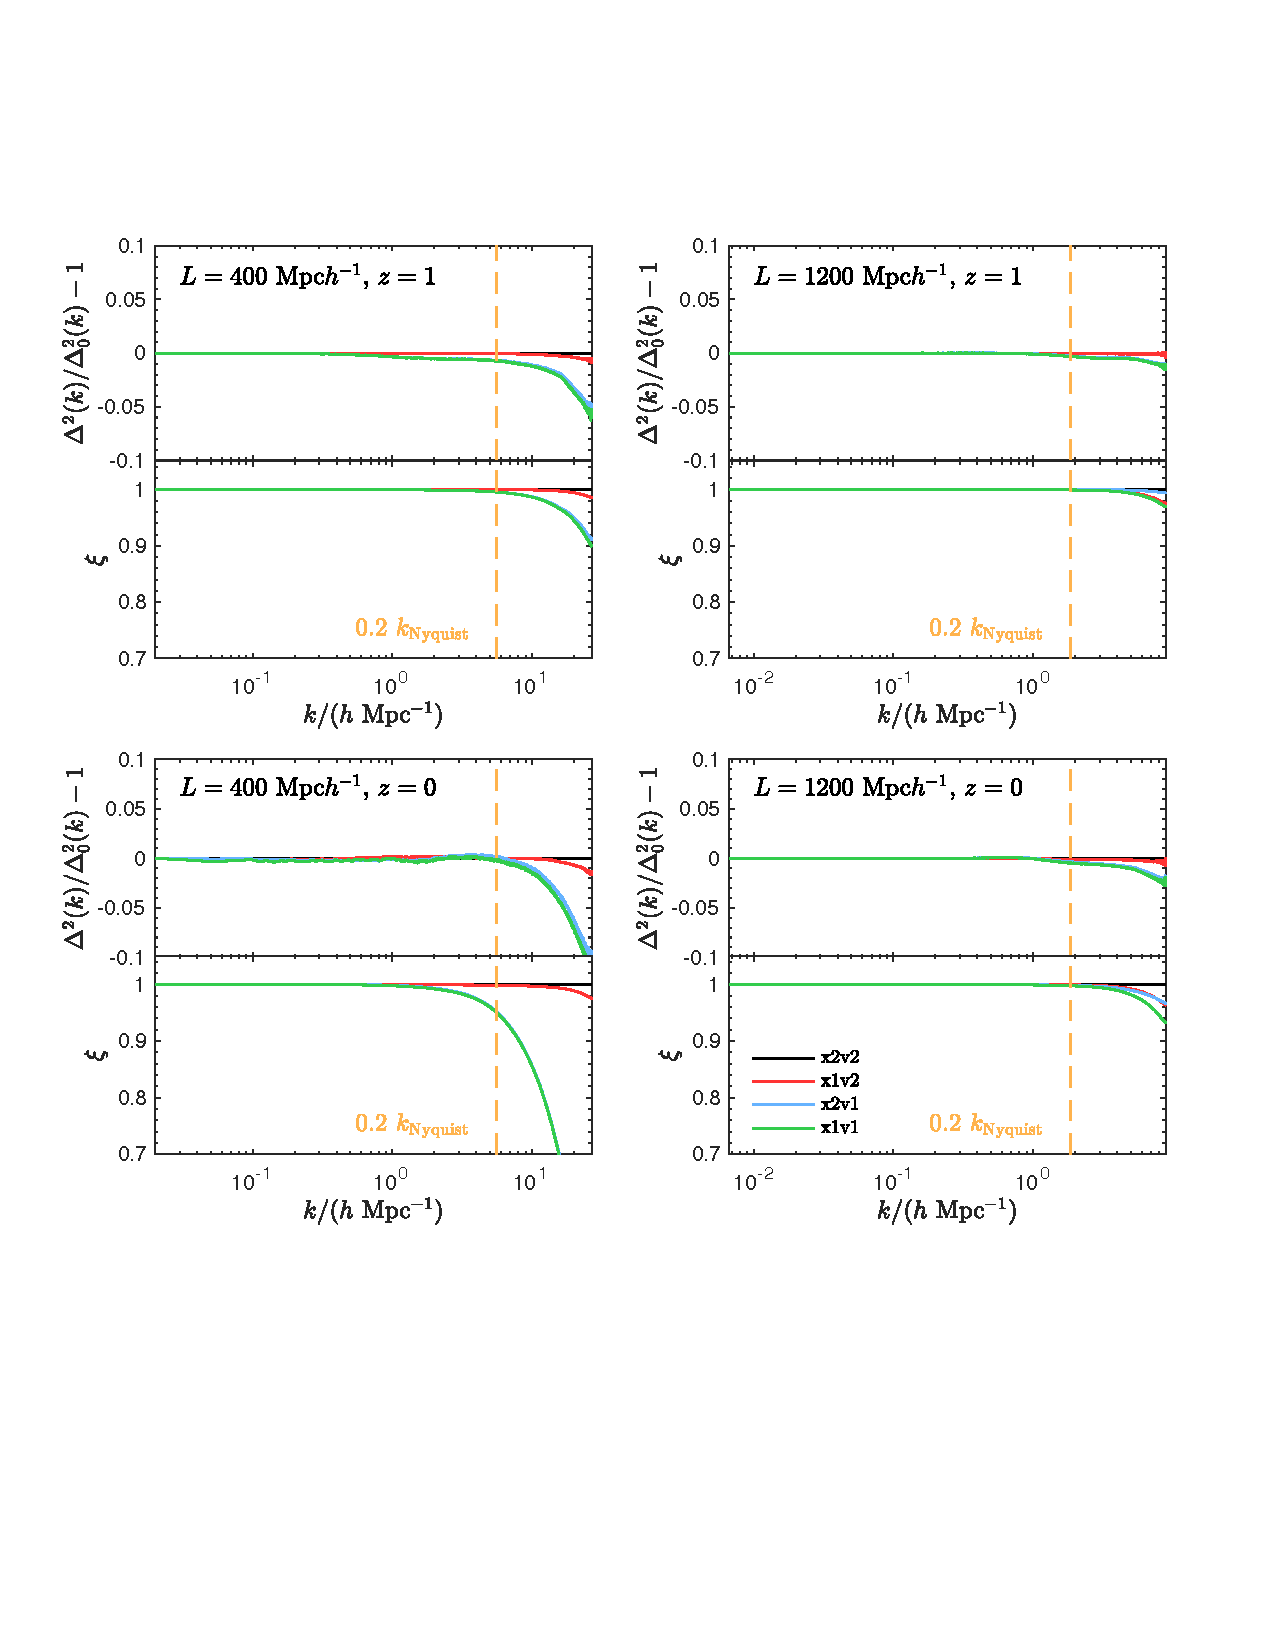
\includegraphics[width=1.1\linewidth]{diff_power.pdf}
 \caption{Fractional error on power spectrum and cross correlations.}
\label{fig.ccc}
\end{figure}

 Cosmological simulation, PM method.

PID.

Summarize memory.

Phi, GPU.


\clearpage

\appendix

\section{A. Initial condition generator}


\acknowledgements

\bibliographystyle{hapj}
\bibliography{haoran_ref}

\end{document}
